% Options for packages loaded elsewhere
\PassOptionsToPackage{unicode}{hyperref}
\PassOptionsToPackage{hyphens}{url}
%
\documentclass[
]{article}
\usepackage{lmodern}
\usepackage{amssymb,amsmath}
\usepackage{ifxetex,ifluatex}
\ifnum 0\ifxetex 1\fi\ifluatex 1\fi=0 % if pdftex
  \usepackage[T1]{fontenc}
  \usepackage[utf8]{inputenc}
  \usepackage{textcomp} % provide euro and other symbols
\else % if luatex or xetex
  \usepackage{unicode-math}
  \defaultfontfeatures{Scale=MatchLowercase}
  \defaultfontfeatures[\rmfamily]{Ligatures=TeX,Scale=1}
\fi
% Use upquote if available, for straight quotes in verbatim environments
\IfFileExists{upquote.sty}{\usepackage{upquote}}{}
\IfFileExists{microtype.sty}{% use microtype if available
  \usepackage[]{microtype}
  \UseMicrotypeSet[protrusion]{basicmath} % disable protrusion for tt fonts
}{}
\makeatletter
\@ifundefined{KOMAClassName}{% if non-KOMA class
  \IfFileExists{parskip.sty}{%
    \usepackage{parskip}
  }{% else
    \setlength{\parindent}{0pt}
    \setlength{\parskip}{6pt plus 2pt minus 1pt}}
}{% if KOMA class
  \KOMAoptions{parskip=half}}
\makeatother
\usepackage{xcolor}
\IfFileExists{xurl.sty}{\usepackage{xurl}}{} % add URL line breaks if available
\IfFileExists{bookmark.sty}{\usepackage{bookmark}}{\usepackage{hyperref}}
\hypersetup{
  hidelinks,
  pdfcreator={LaTeX via pandoc}}
\urlstyle{same} % disable monospaced font for URLs
\usepackage{longtable,booktabs}
% Correct order of tables after \paragraph or \subparagraph
\usepackage{etoolbox}
\makeatletter
\patchcmd\longtable{\par}{\if@noskipsec\mbox{}\fi\par}{}{}
\makeatother
% Allow footnotes in longtable head/foot
\IfFileExists{footnotehyper.sty}{\usepackage{footnotehyper}}{\usepackage{footnote}}
\makesavenoteenv{longtable}
\usepackage{graphicx}
\makeatletter
\def\maxwidth{\ifdim\Gin@nat@width>\linewidth\linewidth\else\Gin@nat@width\fi}
\def\maxheight{\ifdim\Gin@nat@height>\textheight\textheight\else\Gin@nat@height\fi}
\makeatother
% Scale images if necessary, so that they will not overflow the page
% margins by default, and it is still possible to overwrite the defaults
% using explicit options in \includegraphics[width, height, ...]{}
\setkeys{Gin}{width=\maxwidth,height=\maxheight,keepaspectratio}
% Set default figure placement to htbp
\makeatletter
\def\fps@figure{htbp}
\makeatother
\setlength{\emergencystretch}{3em} % prevent overfull lines
\providecommand{\tightlist}{%
  \setlength{\itemsep}{0pt}\setlength{\parskip}{0pt}}
\setcounter{secnumdepth}{-\maxdimen} % remove section numbering

\author{}
\date{}

\begin{document}

\begin{center}\rule{0.5\linewidth}{0.5pt}\end{center}

title = "Master recipe: How to learn your machines"\\
menuTitle = "How to learn your machines"\\
draft = false\\
weight=11

\begin{center}\rule{0.5\linewidth}{0.5pt}\end{center}

These are notes I made while I was taking the \url{Deeplearning.ai}
\href{https://www.coursera.org/specializations/deep-learning}{Deep
Learning Specialization}, more specifically, the awesome
\href{https://www.coursera.org/learn/deep-neural-network}{Improving Deep
Neural Networks}: Hyperparameter tuning, Regularization and Optimization
course, through which Andrew Ng lays down a basic recipe for training
your machines! I highly recommend you taking it, \textbf{it's free} and
you'll absolutely learn something even if you're an experienced ML
practicioner.

\{\{\% notice tip \%\}\}

This may very well be the most useful part of my project. Be sure to at
least take a look. 🙂

\{\{\% /notice \%\}\}

\hypertarget{header-n8}{%
\subsection{Preparing your data}\label{header-n8}}

One of the first questions while preparing you should answer is
\textbf{how to split your dataset?} One good practice is to split the
data into three parts;

\hypertarget{header-n10}{%
\paragraph{\texorpdfstring{\textbf{Training set, cross validation/dev
set and test
set.}}{Training set, cross validation/dev set and test set.}}\label{header-n10}}

\begin{center}\rule{0.5\linewidth}{0.5pt}\end{center}

\begin{figure}
\centering
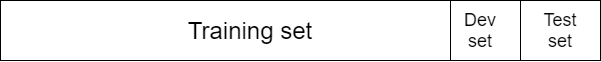
\includegraphics{/images/ai/data.png}
\caption{}
\end{figure}

\begin{itemize}
\item
  You train the data on the training set, and validate it using the dev
  set.
\item
  Since you're using the dev set to tune the model hyperparameters,
  you're kinda fitting them to the data in the dev set. That's why after
  you've chosen the exact hyperparameters you want and after you've
  completely trained your model, you should test it using the test set,
  which is data it has never ever seen before, and should give you a
  "real-world" benchmark on how it performs.
\end{itemize}

\hypertarget{header-n18}{%
\paragraph{\texorpdfstring{\textbf{How to split the data
(size-wise):}}{How to split the data (size-wise):}}\label{header-n18}}

\begin{center}\rule{0.5\linewidth}{0.5pt}\end{center}

\begin{itemize}
\item
  If you have a small amount of data, in the tens of thousands, you can
  use the "olden" way (pre big-data) of splitting the data: 60\% for
  your training set, 20\% for your dev and 20\% for your test set
\item
  If however your data is in the millions, using 20\% or 200 000
  examples for your dev and test is surely a bit of an overkill. You can
  decide to use something like 10 000 examples for your dev/test sets,
  so you'd have a split of 99\%/1\%/1\% for your train/dev/test sets
  respectively.
\item
  If your dataset is even bigger, you can also use something like
  99.5\%/0.4\%/0.1\%, whatever lets you quickly decide how well the
  model is training and performing on data it's never seen before.
\end{itemize}

\hypertarget{header-n27}{%
\paragraph{\texorpdfstring{\textbf{Make sure your training and dev/test
sets come from the same
distribution.}}{Make sure your training and dev/test sets come from the same distribution.}}\label{header-n27}}

\begin{center}\rule{0.5\linewidth}{0.5pt}\end{center}

\begin{itemize}
\item
  If your training data is really high res, but the data you'll use
  during inference is lower quality due to lower resolutions, shaky
  camera, dirty lenses, and so on, your model won't perform well.
\item
  Your training data should be as similar as possible to real world data
  you'll use during inference, and you should try to cover as much
  possible situations you can, which includes different weather
  conditions, bumpy roads, and so on.
\item
  The main reason for this type of mismatch is that you don't have
  enough training data, so you get some online, e.g. if you took a
  YouTube video of a car driving around town that has a super high res
  camera and added it to your training data, but your RC car has a
  really low res camera.
\end{itemize}

\hypertarget{header-n36}{%
\paragraph{\texorpdfstring{\textbf{How to know if your model has high
variance or bias (or
both):}}{How to know if your model has high variance or bias (or both):}}\label{header-n36}}

\begin{center}\rule{0.5\linewidth}{0.5pt}\end{center}

\textbf{Here's a great illustration by Andrew Ng} on what high bias and
variance look like:

\begin{figure}
\centering
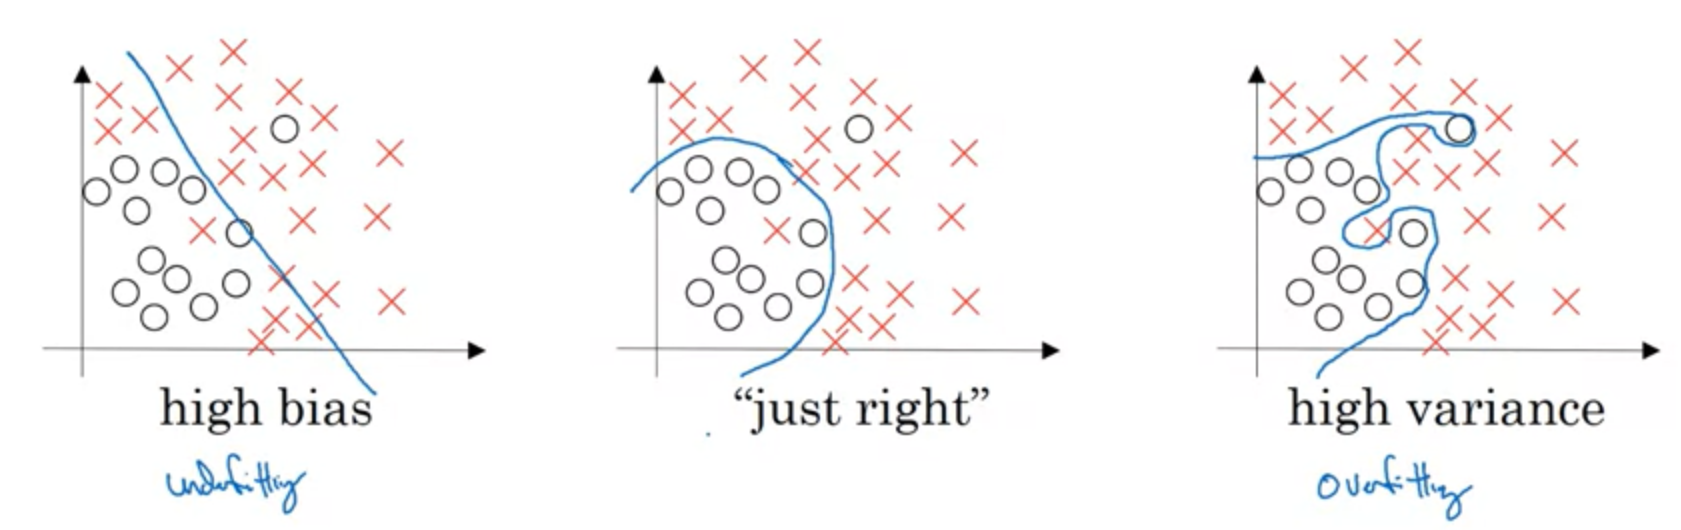
\includegraphics{/images/howtotrain/biasvariance.png}
\caption{}
\end{figure}

\begin{itemize}
\item
  \textbf{High variance:} the model is overfitting the training data and
  performing poorly on new unseen data.
\item
  \textbf{High bias:} the model isn't even performing well on the
  training data.
\item
  \textbf{High bias and high variance:} the model underfits the training
  data but performs even worse on the dev data.
\end{itemize}

\textbf{The two key things to take away are:}

\begin{itemize}
\item
  By looking at how well the model performs on the training data, you
  can see how much bias it has; if it has a low error, it has a low
  bias, if it has a large error, it has large bias.
\item
  By looking at how well the model performs on the dev set, you can see
  how much variance it has; if it performs much worse than on the
  training set, it has high variance, if it performs slightly worse or
  the same, it has low variance and generalizes well.
\end{itemize}

\hypertarget{header-n53}{%
\section{Basic recipe for learning your machines}\label{header-n53}}

\begin{itemize}
\item
  Get the model to perform well on the training data (low bias)
\item
  Get the model to perform well on the dev set data (low variance)
\end{itemize}

\hypertarget{header-n59}{%
\paragraph{\texorpdfstring{\textbf{If you have large
bias:}}{If you have large bias:}}\label{header-n59}}

\begin{center}\rule{0.5\linewidth}{0.5pt}\end{center}

\begin{itemize}
\item
  (Almost always works): Try a bigger network: more hidden layers, more
  hidden units.
\item
  (Sometimes works, but never hurts): Try training it longer: give it
  more time or use more advanced optimization algorithms.
\item
  (Maybe it'll work, maybe it won't): Try finding a better neural net
  architecture: try finding an architecture that's proven to work for
  your specific problem.
\item
  Consider asking yourself: is this even possible to do? If you're
  trying to train a classifier on very blurry low res images, is it even
  possible to do so? What's the base error for that problem?
\end{itemize}

\textbf{If you have large variance:}

\begin{itemize}
\item
  (Best way to solve it): Get more data, it can only help. But sometimes
  it's impossible to get more data.
\item
  (Almost always helps): Regularization
\item
  (Maybe it'll work, maybe it won't): Try finding a better neural net
  architecture. Same as for the large bias problem.
\end{itemize}

\textbf{Don't worry about the bias-variance tradeoff if you're doing
deep learning. It isn't much of a thing anymore:}

\begin{itemize}
\item
  As long as you can train a bigger network (and use regularization),
  you'll almost certainly be able to get rid of high bias without
  increasing variance (by much).
\item
  As long as you can get more data (not always, but mostly possible),
  you'll almost certainly be able to get rid of high variance without
  increasing bias (by much).
\end{itemize}

\hypertarget{header-n84}{%
\paragraph{\texorpdfstring{\textbf{Regularizing neural
nets}}{Regularizing neural nets}}\label{header-n84}}

\begin{center}\rule{0.5\linewidth}{0.5pt}\end{center}

To try and gain some intuition about regularization in neural nets,
let's walk through implementing L2 regularization in a neural net. Since
we're mostly doing computer vision stuff with our self-driving car,
we'll most likely be using batch normalization and dropout
regularization rather than L2, which is used much more often in computer
vision, so feel free to skip this part if you're not interested.

If our cost function is defined as:

We can regularize it by adding a regularization term:

Let's break it down.

The first part uses the regularization parameter \(\lambda\), which is a
hyperparameter to be tuned using the dev set, and divides it by \(2n\),
which is just a scaling constant.

The second part uses
\href{http://mathworld.wolfram.com/FrobeniusNorm.html}{the Frobenius
norm} (basically the L2 norm of a matrix), and it basically sums up the
squares of all the elements of all \(\mathcal{w}\) matrices we use:

\(\mathcal{w}\) is a \((n^{[l]}, n^{[l-1]})\) dimensional matrix, where
the first dimension represents the number of units in the \(l\)-th
layer, and the second represents the number of units in the previous
layer.

When implemented, during backprop the \(W^{[l]}\) matrix gets multiplied
by \(\frac{\lambda}{n}\), a number slightly smaller than 1, which is why
it's also called weight decay, since the weight loses just a bit of it's
value.

\hypertarget{header-n97}{%
\paragraph{\texorpdfstring{\textbf{Why does this
help?}}{Why does this help?}}\label{header-n97}}

\begin{center}\rule{0.5\linewidth}{0.5pt}\end{center}

If we set the \(\lambda\) parameter in the regularization term below to
a large value, it will set the values of \(w^{[l]}\) very close to zero.

So what happens if \(w^{[l]}\) is close to zero? It will cause
\(z^{[l]}\) to have a very small range of values, close to zero.

Let's assume we're using \(tanh(z)\) as our activation function.

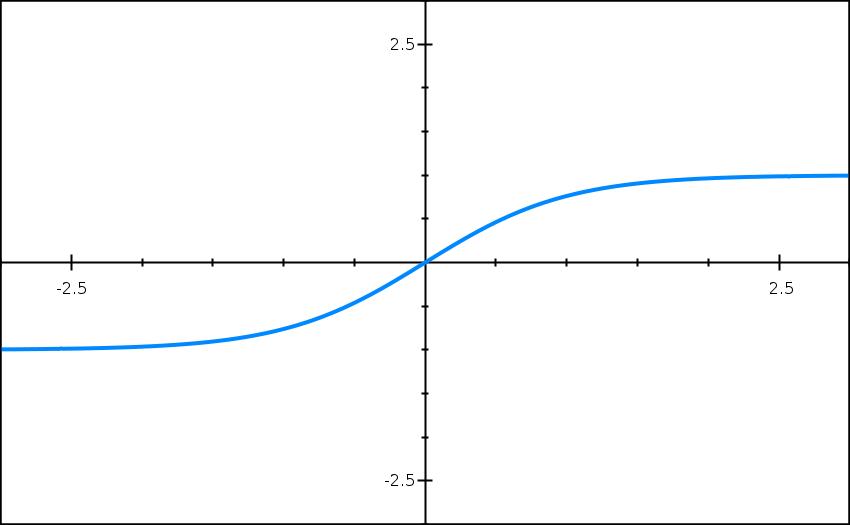
\includegraphics{/images/howtotrain/tanh1.png}

If the value of \(z^{[l]}\) can be only a small range of values close to
zero, our activation function will start looking like a linear function,
as shown below:

\begin{figure}
\centering
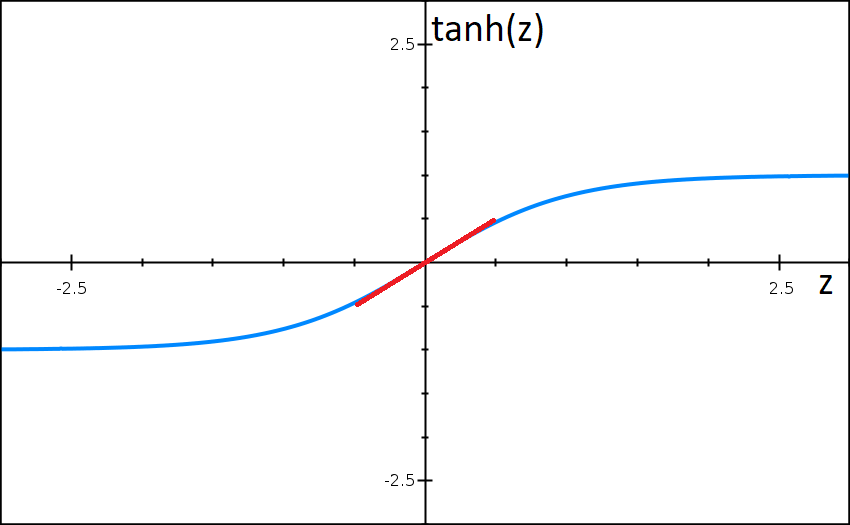
\includegraphics{/images/howtotrain/tanh2.png}
\caption{image-20191126153603629}
\end{figure}

Which in turn means every layer in our neural net will begin to look
like a linear layer, which will cause our network to be able to
approximate only a linear function to our data, which will cause our
model to go from high variance to high bias.

Of course, we don't (and won't) set our \(\lambda\) parameter to a very
large value, but rather set it to somewhere in between, which will get
rid of our high variance problem and not cause high bias instead.

\hypertarget{header-n109}{%
\paragraph{\texorpdfstring{\textbf{Dropout
regularization}}{Dropout regularization}}\label{header-n109}}

\begin{center}\rule{0.5\linewidth}{0.5pt}\end{center}

\textbf{This illustration was also taken from Andrew Ng's course video}:

\begin{figure}
\centering
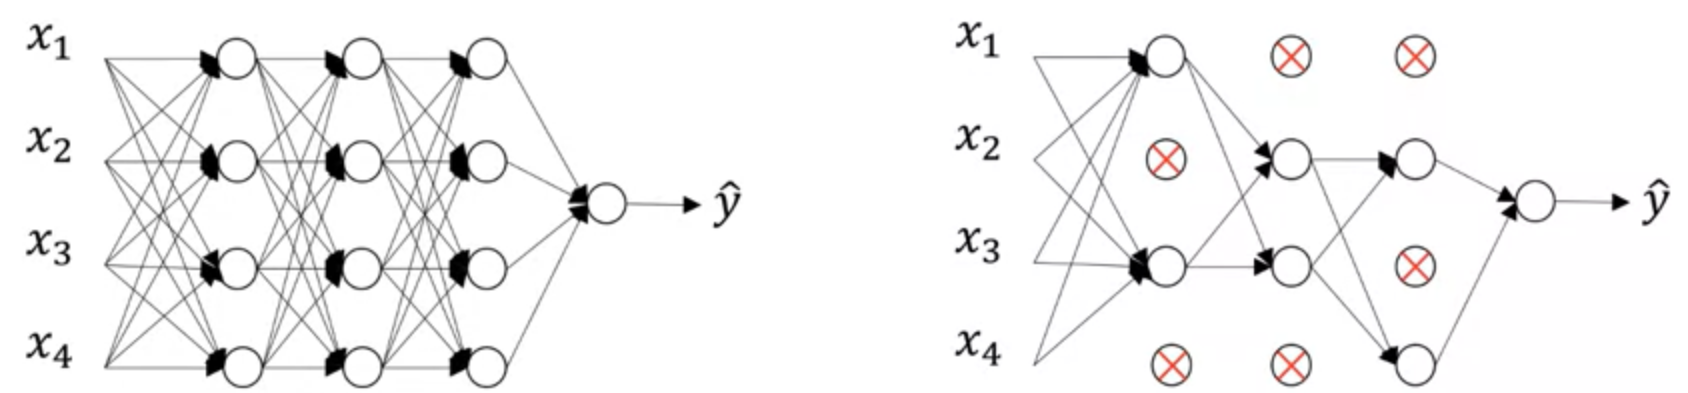
\includegraphics{/images/howtotrain/dropout.png}
\caption{}
\end{figure}

Imagine we have a neural net that looks like the one pictured above, on
the left.

\textbf{To stop our model from overfitting our data, we can randomly
knock-out some neurons while training our model.} This in turn causes
the model to be unable to rely on just a particular set of neurons, or a
pathway of neurons, so it has to train multiple subsets of neural nets,
which makes it much more difficult to overfit the data, since it never
knows when some of the neurons will be knocked out.

\hypertarget{header-n115}{%
\subsection{Other tips to prevent overfitting/bias}\label{header-n115}}

\hypertarget{header-n116}{%
\paragraph{\texorpdfstring{\textbf{Augment your
data}}{Augment your data}}\label{header-n116}}

\begin{center}\rule{0.5\linewidth}{0.5pt}\end{center}

Let's say we're training our car on the following track:

\begin{figure}
\centering
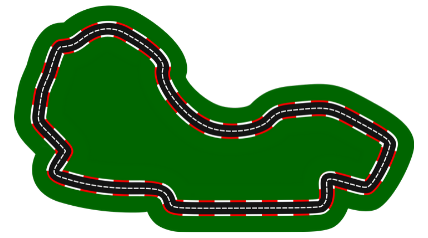
\includegraphics{/images/howtotrain/firstTrack.png}
\caption{}
\end{figure}

We run a few laps on the track and save our data. If we've only driven
in the usual, counter-clockwise direction, we have inadvertently caused
our model to be slightly biased to always turn a bit to the left.

Why?

\begin{figure}
\centering
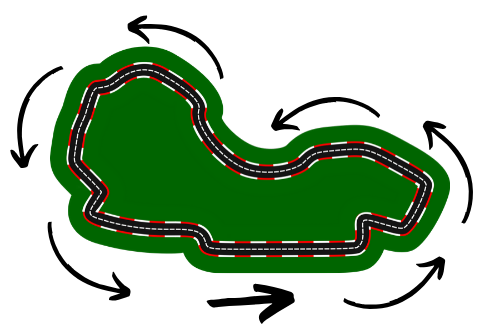
\includegraphics{/images/howtotrain/trackCounter.png}
\caption{}
\end{figure}

We can see that, globally, the car is always turning a bit to the left.
So if you only include this data in your training set, the car will
always be inclined to turn just a bit to the left.

\hypertarget{header-n124}{%
\paragraph{\texorpdfstring{\textbf{How to solve
it}}{How to solve it}}\label{header-n124}}

\begin{center}\rule{0.5\linewidth}{0.5pt}\end{center}

Other than driving the very same track, just in the opposite direction,
you can simply mitigate this issue by augmenting your data with the same
images, just horizontally flipped, thus getting:

\begin{figure}
\centering
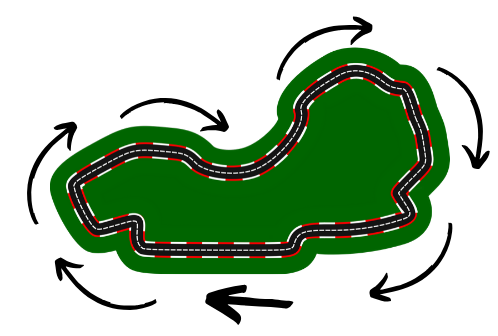
\includegraphics{/images/howtotrain/trackClockwise.png}
\caption{}
\end{figure}

Now your car shouldn't be inclined much to steer to one side or the
other for no reason.

\{\{\% notice info \%\}\}

Make sure to make copies of your JSON files and invert their steering
values as well.

\{\{\% /notice \%\}\}

\hypertarget{header-n132}{%
\paragraph{\texorpdfstring{\textbf{Augmentation by Neural Style
transfer}}{Augmentation by Neural Style transfer}}\label{header-n132}}

\begin{center}\rule{0.5\linewidth}{0.5pt}\end{center}

You can even apply preprocessing like this to your images to try and
make it focus on the more important features such as lane lines:

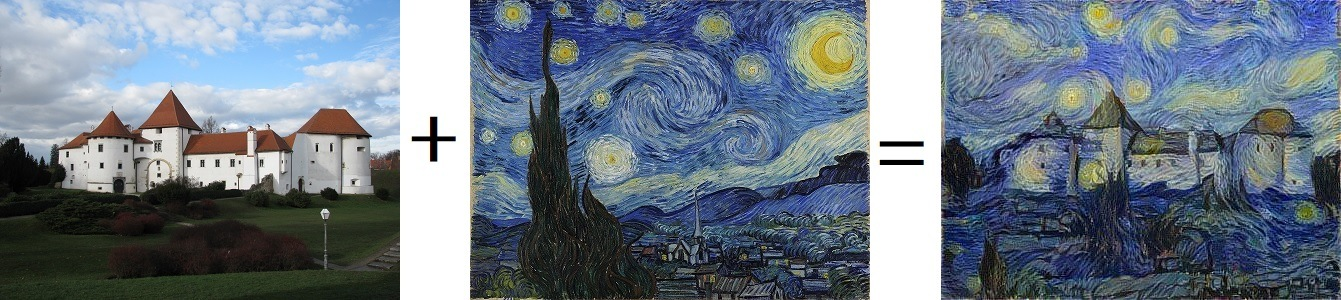
\includegraphics{/images/ai/vangogh.jpg}\\
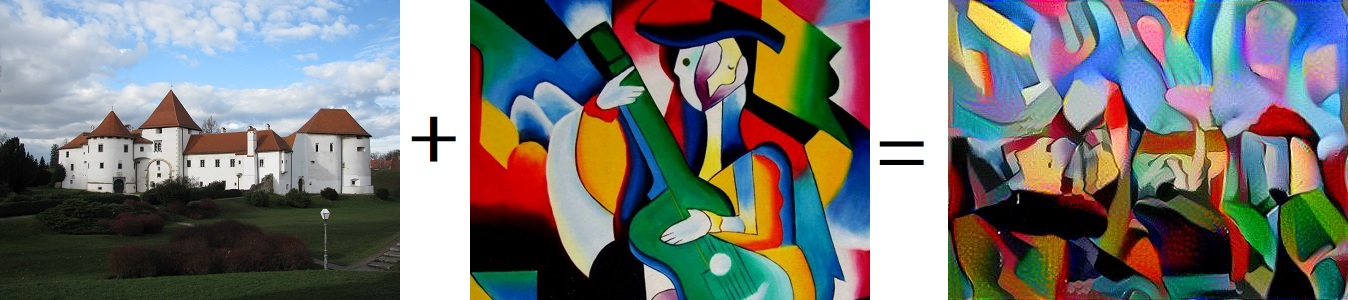
\includegraphics{/images/ai/picasso.jpg}

\hypertarget{header-n136}{%
\paragraph{\texorpdfstring{\textbf{Also, I wrote this just to have an
excuse to make some artful Baby Yoda memes, which had to be put into
this project somehow, so here
goes:}}{Also, I wrote this just to have an excuse to make some artful Baby Yoda memes, which had to be put into this project somehow, so here goes:}}\label{header-n136}}

\begin{center}\rule{0.5\linewidth}{0.5pt}\end{center}

\includegraphics{/images/howtotrain/babyyoder1.jfif}\\
\includegraphics{/images/howtotrain/babyyoder2.jfif}\\
\includegraphics{/images/howtotrain/babyyoder3.jfif}

\textbf{You could still tell that it's Baby Yoda, even though the images
lost a lot of the original information about him, e.g. the hairs on his
head.} So in contrast, you could use this approach and still be able to
identify lane lines on images, but just by focusing on the things that
make us recognize them the most.

Or not. Anyways, artful Baby Yoda memes.

\hypertarget{header-n141}{%
\paragraph{\texorpdfstring{\textbf{Early
stopping}}{Early stopping}}\label{header-n141}}

\begin{center}\rule{0.5\linewidth}{0.5pt}\end{center}

When training your model, you can often see the validation error getting
lower over time, following the training error curve, but then at one
moment you see it take off and get much worse over time:

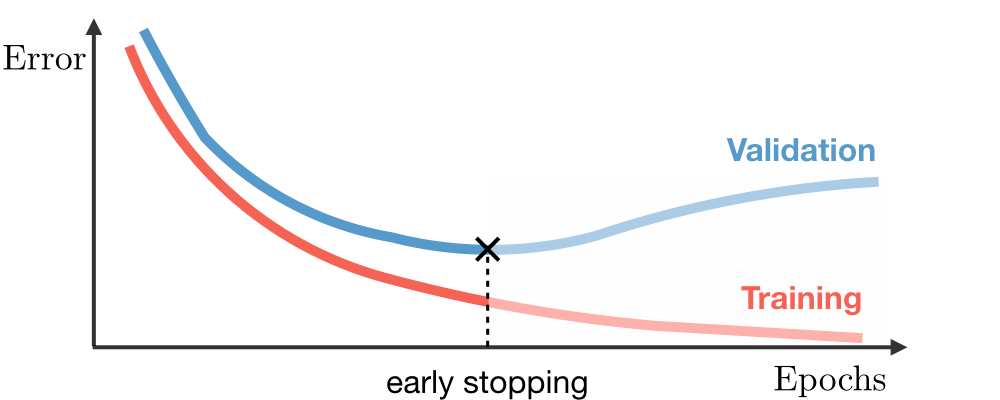
\includegraphics{/images/howtotrain/early-stopping.png}

\textbf{One possible solution is stopping the training early, when you
see the validation error starting to increase.}

\textbf{\underline{Just keep in mind that by doing so, you're now
coupling two optimization problems that you were solving as separate
before}}: the optimization of your cost function and the prevention of
overfitting the dataset. By doing so, you're not doing quite the best
job you could at minimizing the cost function, since it's obvious that
the error could get much lower if the training wasn't stopped early,
while you're simultaneously trying not to overfit your data.

One alternative could be using L2 regularization or some other
regularization technique, but you can often see early stopping being
used in practice. Just keep in mind the trade off you're doing.

\hypertarget{header-n148}{%
\paragraph{\texorpdfstring{\textbf{Iterating quicker: a single number
performance
metric}}{Iterating quicker: a single number performance metric}}\label{header-n148}}

\begin{center}\rule{0.5\linewidth}{0.5pt}\end{center}

First, lets define two terms using a classifier example; precision and
recall.

\textbf{Precision:} of the examples that your classifier recognizes as
X, how many examples actually are X.\\
\textbf{Recall:} of the examples that are actually X, how many of them
does your classifier recognize as X.

We can combine these two metrics into a single number, as a
\href{https://www.wikiwand.com/en/Harmonic_mean}{harmonic mean} of the
two, which is called \href{https://www.wikiwand.com/en/F1_score}{the F1
score}:

But why?\\
Sure, this doesn't help much if you're just using a binary classifier
like mentioned above, to see if something is X or not. Or even if you're
classifying things into two classes.

But imagine trying to decide between three implementations of a
classifier with 3 possible classes:

\begin{longtable}[]{@{}lllllll@{}}
\toprule
Implementation/Classes & A (precision) & A (recall) & B (precision) & B
(recall) & C (precision) & C (recall)\tabularnewline
\midrule
\endhead
First implementation & 95\% & 90\% & 89\% & 88\% & 92\% &
89\%\tabularnewline
Second implementation & 93\% & 89\% & 92\% & 90\% & 92\% &
90\%\tabularnewline
Third implementation & 89\% & 88\% & 95\% & 93\% & 90\% &
89\%\tabularnewline
\bottomrule
\end{longtable}

Which one is the best? Sure isn't easy to tell from the table above. At
least not to me.

Now look what it would look like if we used the F1 score for all of the
possible classes:

\begin{longtable}[]{@{}llll@{}}
\toprule
Implementation/Classes & A (\(F_1\) score) & B (\(F_1\) score) & C
(\(F_1\) score)\tabularnewline
\midrule
\endhead
First implementation & 92.4\% & 88.5\% & 90.5\%\tabularnewline
Second implementation & 91\% & 91\% & 91\%\tabularnewline
Third implementation & 88.5\% & 94\% & 89.5\%\tabularnewline
\bottomrule
\end{longtable}

Looks much simpler than the first table, but still could be simpler.
Since we're probably interested in our classifier working as best as
possible over all classes, we can take the average of all of the 3
\(F_1\) scores to get one simple number that tells us how well our
classifier works:

\begin{longtable}[]{@{}ll@{}}
\toprule
Implementation/Classes & Average \(F_1\) score\tabularnewline
\midrule
\endhead
First implementation & 90.5\%\tabularnewline
Second implementation & 91\%\tabularnewline
Third implementation & 90.7\%\tabularnewline
\bottomrule
\end{longtable}

\hypertarget{header-n226}{%
\paragraph{\texorpdfstring{\textbf{Why do
this?}}{Why do this?}}\label{header-n226}}

\begin{center}\rule{0.5\linewidth}{0.5pt}\end{center}

The example above could've easily had a hundred different classes, with
a dozen different implementations. That would've been impossible to look
at even if you used \(F_1\) scores for every class.

When trying out a bunch of different values of hyperparameters and
implementation details, it's much faster to iterate and much easier to
decide between all possible implementations when you have a single
number that tells you how well it performs. And I believe this is a
pretty good way to get one, even considering the amount of some
fine-grained details you lose. You can always look them up after you
eliminate some implementations, and have only a few you're actually
considering.

\hypertarget{header-n230}{%
\paragraph{\texorpdfstring{One important thing to notice is that
\textbf{there could be other important metrics to look at} other than
how accurate our classifier
is.}{One important thing to notice is that there could be other important metrics to look at other than how accurate our classifier is.}}\label{header-n230}}

\begin{center}\rule{0.5\linewidth}{0.5pt}\end{center}

For an example, we could be making a classifier that classifies
obstacles our car will collide with if we don't avoid them. Surely, we'd
like to correctly classify as much of those as possible, so make a
table, as the one above:

\begin{longtable}[]{@{}ll@{}}
\toprule
Classifier/Score & \(F_1\) score\tabularnewline
\midrule
\endhead
First classifier & 92\%\tabularnewline
Second classifier & 97\%\tabularnewline
Third classifier & 99\%\tabularnewline
\bottomrule
\end{longtable}

Cool, so we pick the third classifier. \textbf{And our car crashes.}
Wait, wut?

We picked the best classifier in terms of it correctly classifying as
much of the objects in our path as possible, but \textbf{there's one
thing we didn't look at;} \textbf{the time it takes it to classify an
object.}

\begin{longtable}[]{@{}lll@{}}
\toprule
Classifier/Score & \(F_1\) score & Average runtime\tabularnewline
\midrule
\endhead
First classifier & 92\% & 20 ms\tabularnewline
Second classifier & 97\% & 70 ms\tabularnewline
Third classifier & 99\% & 3000 ms\tabularnewline
\bottomrule
\end{longtable}

So yeah, we did recognize most of the objects we were on a collision
path with, but by the time that we did, the car had already crashed into
them.

Taking that in mind, the second classifier is obviously the better
choice.

So it's important to keep in mind that while we're trying to optimize
one of the metrics of our model, we also have to pay attention to the
other minimum requirements the model must have in order to actually be
usable in the real world, as per our real-time necessary example.

\hypertarget{header-n268}{%
\paragraph{\texorpdfstring{\textbf{Choosing
Hyperparameters}}{Choosing Hyperparameters}}\label{header-n268}}

\begin{center}\rule{0.5\linewidth}{0.5pt}\end{center}

\textbf{Hyperparameters ordered by importance are:}

\begin{itemize}
\item
  learning rate (alpha)
\item
  beta, number of hidden units, mini-batch size
\item
  number of layers, learning rate decay
\end{itemize}

\textbf{A traditional way to choose hyperparameters is to sample them
from a grid:}

First we'd define a grid, which can either be a randomized or a regular
grid, and then iteratively sample the parameters from it:

\textbf{Illustration by Andrew Ng:}

\begin{figure}
\centering
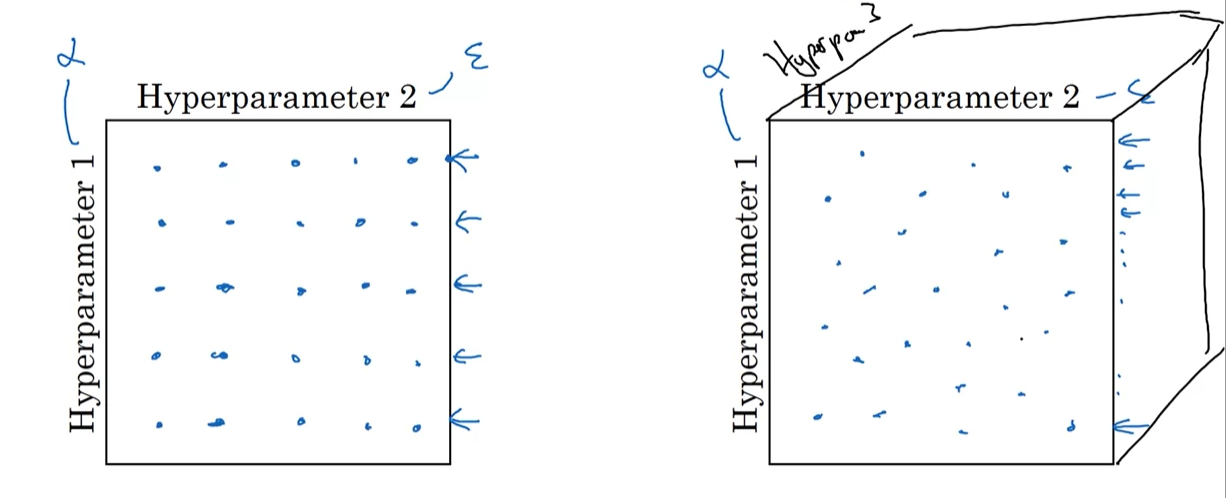
\includegraphics{/images/howtotrain/hyperparameters.png}
\caption{}
\end{figure}

Keep in mind that the grid search approach suffers from
\textbf{\href{https://www.wikiwand.com/en/Curse_of_dimensionality}{the
curse of dimensionality}}.

There's a lot of ways to do this, most frameworks even have built-in
ways of doing this so I'd highly recommend you look into the topic of
\textbf{\href{https://www.wikiwand.com/en/Hyperparameter_optimization}{hyperparameter
optimization}}.

\hypertarget{header-n284}{%
\paragraph{\texorpdfstring{\textbf{Hyperparameters can get
stale}}{Hyperparameters can get stale}}\label{header-n284}}

\begin{center}\rule{0.5\linewidth}{0.5pt}\end{center}

Also keep in mind that you should re-evaluate your hyperparameters every
once in a while, because as you get a lot more data, \textbf{they can
get stale}.

They can also get stale if you get a new GPU/CPU, change your network a
bit or for any number of reasons. Just re-evaluate them from time to
time, depending on how much you're changing stuff around.

\hypertarget{header-n288}{%
\paragraph{Closing thoughts}\label{header-n288}}

\begin{center}\rule{0.5\linewidth}{0.5pt}\end{center}

The more you do this stuff, the easier it'll get, and the more tricks
you'll learn.

The thing about ML is that you have to rely on your intuition a lot. If
a model is misbehaving, you can't simply set a breakpoint on it and
debug it, there can be a plethora of reasons for it:

\begin{itemize}
\item
  Maybe your data is bad
\item
  Maybe there is a bug in your architecture
\item
  Maybe you're just using the wrong hyperparameters
\item
  ...
\end{itemize}

You have to keep trying and not give up. It can take a few days even to
get your model to perform well, even on smaller testing datasets,
depending on the complexity of the task you're trying to achieve.

Do your best to make sure that the things that you can control, e.g. the
quality of your data and its distribution, are okay.

For the parts you can't directly see, like how your convolutional layers
are doing stuff, you can use all sorts of tools like the visualization
techniques we've done earlier to try and gain some intuition on how it's
performing and what could go wrong.

That's pretty much it! Have fun experimenting with your model.

Next up: learning behaviours, e.g. lane changing!

\end{document}
